%%% License: Creative Commons Attribution Share Alike 4.0 (see https://creativecommons.org/licenses/by-sa/4.0/)


%%%%%%%%%%%%%%%%%%%%%%%%%%%%%%%%%%%%%%%%%

%----------------------------------------------------------------------------------------
%	PACKAGES AND OTHER DOCUMENT CONFIGURATIONS
%----------------------------------------------------------------------------------------

\documentclass[a4paper]{article}

\usepackage{amssymb}
\usepackage{enumerate}
\usepackage[usenames,dvipsnames]{color}
\usepackage{fancyhdr} % Required for custom headers
\usepackage{lastpage} % Required to determine the last page for the footer
\usepackage{extramarks} % Required for headers and footers
\usepackage[usenames,dvipsnames]{color} % Required for custom colors
\usepackage{graphicx} % Required to insert images
\usepackage{listings} % Required for insertion of code
\usepackage{courier} % Required for the courier font
\usepackage[table]{xcolor}
\usepackage{amsfonts,amsmath,amsthm,parskip,setspace,url}
\usepackage[section]{placeins}
\usepackage[a4paper]{geometry}
\usepackage[USenglish]{babel}
\usepackage[utf8]{inputenc}
\usepackage{tikz}


% Margins
\topmargin=-0.45in
\evensidemargin=0in
\oddsidemargin=0in
\textwidth=6.5in
\textheight=9.0in
\headsep=0.6in

\linespread{1.1} % Line spacing



%----------------------------------------------------------------------------------------
%   FORMATTING
%----------------------------------------------------------------------------------------
% Set up the header and footer
\pagestyle{fancy}
\lhead[c]{\textbf{{\color[rgb]{.5,0,0} K{\o}benhavns\\Universitet }}} % Top left header
\chead{\textbf{{\color[rgb]{.5,0,0} \Class }}\\ \hmwkTitle  } % Top center head
\rhead{\instructor \\ \theprofessor} % Top right header
\lfoot{\lastxmark} % Bottom left footer
\cfoot{} % Bottom center footer
\rfoot{Page\ \thepage\ of\ \protect\pageref{LastPage}} % Bottom right footer
\renewcommand\headrulewidth{0.4pt} % Size of the header rule
\renewcommand\footrulewidth{0.4pt} % Size of the footer rule


% Other formatting stuff
%\setlength\parindent{12pt}
\setlength{\parskip}{5 pt}
%\theoremstyle{definition} \newtheorem{ex}{\textbf{\Large{Exercise & #}\\}}
\usepackage{titlesec}
\titleformat{\section}[hang]{\normalfont\bfseries\Large}{Problem \thesection:}{0.5em}{}




%----------------------------------------------------------------------------------------
%	NAME AND CLASS SECTION
%----------------------------------------------------------------------------------------
\newcommand{\hmwkTitle}{Exercises for Lecture 5 (M2)} % Assignment title
\newcommand{\Class}{Mechanism Design} % Course/class
\newcommand{\instructor}{Fall 2021} % TA
\newcommand{\theprofessor}{Prof. Egor Starkov} % Professor




%----------------------------------------------------------------------------------------
%   SOLUTIONS
%----------------------------------------------------------------------------------------
\newif\ifsolutions
%\solutionstrue




\begin{document}

\begin{center}
		\LARGE\textbf{Exercises for Lecture 5 (M2):\\ AGV. Social choice.}
\end{center}



\section{Transfers and Social choice}
% MWG 21.B.3
% social choice
Consider a public good provision problem, with $k \in \{0,1\}$. The society consists of $N$ agents (for simplicity suppose $N$ is odd) with Euclidean preferences and valuations $(\theta_1, ..., \theta_N)$ for the public good (where $\theta_i$ can be positive or negative). The social cost of the public good is zero.

\begin{enumerate}
\item Show that a decision made via the majority voting is Pareto-optimal in the absence of transfers, but generically not Pareto-optimal if transfers are allowed.
\item Compare and contrast the decision yielded by the majority rule (a ``median'') with the Pareto-optimal decision rule when transfers are allowed (a ``mean'').
\end{enumerate}


\ifsolutions
\section*{Solution}
Let $f_M(\theta)$ denote the social choice function corresponding to the majority voting procedure, and $f_T(\theta)$ denote the Pareto-optimal alternative in the presence of transfers. Then
\begin{align*}
f_M(\theta) &= \mathbb{I} \left\{ |Y(\theta)| > |N(\theta)| \right\},
\\
\text{where } Y(\theta) &\equiv \{ i \in N | \theta_i \geq 0 \},
\\
Z(\theta) &\equiv \{ i \in N | \theta_i < 0 \}.
\end{align*}
In words, $f_M(\theta)$ selects $k=1$ if and only if there are more agents preferring alternative $k=1$ (i.e., with $\theta_i \geq 0$) than agents preferring alternative $k=0$ (i.e., with $\theta_i < 0$). To show that this is Pareto-optimal in the absence of transfers, note that the only other option is to select (for some $\theta$) the opposite alternative $k=1-f(\theta)$. This would harm all agents $i \in Y(\theta)$, hence would not be a Pareto-improvement, hence $f(\theta)$ is Pareto-optimal.\footnote{Note that by this logic, any social choice rule is Pareto-optimal in this setting as long as it satisfies unanimity.}

On the other hand, $f_T(\theta)$ is defined to be Pareto-optimal given transfers are alloweed. It is natural to restrict $\sum_{i=1}^{N} t_i = 0$ (or $\leq 0$), since otherwise distributing more transfers is always an improvement. Given this, it is immediate that $f_T(\theta) = \mathbb{I} \{\sum_{i=1}^N \theta_i \geq 0 \}$. This is because if the other $k$ is chosen for some $\theta$, then flipping a decision and redistributing transfers is an improvement.\footnote{If $\sum_{i=1}^N \theta_i \geq 0$ and $f(\theta)=0$ then flipping the decision and increasing every $i$'s transfer by $\theta_i - \varepsilon$ (which can be a negative amount for some $i$) strictly improves all agents' utility and balances the budget for some $\varepsilon > 0$. Conversely, if $\sum_{i=1}^N \theta_i < 0$ and $f(\theta)=1$ then flipping the decision and decreasing transfers by $\theta_i + \varepsilon$ is an improvement by similar logic.}

In other words, treating $(\theta_1,...,\theta_N)$ as a statistical sample, $f_M(\theta)$ selects $k=1$ iff the \emph{median} $\theta_i$ is positive, whereas $f_T(\theta)$ selects $k=1$ whenever the \emph{mean} of all valuations is positive. While for some distributions the two can coincide (e.g., if $\theta_i \in \{-1,1\}$), in general they do not.

Intuitively, the majority rule $f_M$ only counts the number of people in favor of either alternative, but it does not account for the intensity of preferences. Transfers can be used to account for this intensity, reallocating utility from agents with strong preferences to agents who are close to being indifferent between the two options.
\fi 



\section{Social choice with two alternatives}
	Consider a social choice problem between two alternatives in $X = \{l, r\}$ (could be a ``left-leaning policy'' and a ``right-leaning policy'').
	\begin{enumerate}
		\item What \emph{ordinal} preferences (rankings $\succsim_i$) can an individual have over $X$?
		\item Consider a society of two citizens, $i=1,2$ that can have any of the preferences you identified above.
		\begin{enumerate}
			\item Give an example of a social preference $\succsim$ that satisfies the three axioms from class (Full Domain, Unanimity, IIA).
			\item Is it dictatorial? (Note that Arrow's theorem does not apply.)
			\item Do there exist any other social preferences that satisfy the same requirements? Are any/all of them dictatorial?
		\end{enumerate}
		\item Now consider a society of three citizens, $i=1,2,3$. Give an example of a social preference that satisfies the three axioms (A1)-(A3) and is not dictatorial.
	\end{enumerate}

\ifsolutions
\section*{Solution}
	\begin{enumerate}
		\item $l \succsim_i r$, $r \succsim_i l$, and $l \sim_i r$. If you restrict attention to strict rankings (as is sometimes done), then only $l \succ_i r$ and $r \succ_i l$ remain.
		%For simplicity, we suppose from this point onwards either that preferences are strict (so $l \sim_i r$ never occurs), or that in case $l \sim_i r$ player $i$ randomly reports one of the two weak preferences. This is not necessary, and you can do the exercise with indifferences as well.
		
		\item For convenience, encode preferences using types $\theta_i \in \{l,r\}$ so that if $\theta_i=l$ then $l \succsim_i r$ and if $\theta_i=r$ then $r \succsim_i l$. For simplicity, suppose that if $l \sim_i r$ then $i$ randomly reports one of the two weak preferences.
		Then all possible social preferences (ignoring indifferences) are given by the columns of the following table, where each cell indicates the socially preferred option:
		\begin{center}
		\begin{tabular}{c|c c c c c c c c c c c c c c c c|}
			& \multicolumn{16}{c}{$\succsim_S$ (preferred option)}
			\\
			$(\theta_1,\theta_2)$ & 1 & 2 & 3 & 4 & 5 & 6 & 7 & 8 & 9 & 10 & 11 & 12 & 13 & 14 & 15 & 16
			\\ \hline 
			$(l,l)$ & $l$ & $l$ & $l$ & $l$ & $r$ & $l$ & $l$ & $r$ & $l$ & $r$ & $r$ & $l$ & $r$ & $r$ & $r$ & $r$
			\\
			$(l,r)$ & $l$ & $l$ & $l$ & $r$ & $l$ & $l$ & $r$ & $l$ & $r$ & $l$ & $r$ & $r$ & $l$ & $r$ & $r$ & $r$
			\\
			$(r,l)$ & $l$ & $l$ & $r$ & $l$ & $l$ & $r$ & $l$ & $l$ & $r$ & $r$ & $l$ & $r$ & $r$ & $l$ & $r$ & $r$
			\\
			$(r,r)$ & $l$ & $r$ & $l$ & $l$ & $l$ & $r$ & $r$ & $r$ & $l$ & $l$ & $l$ & $r$ & $r$ & $r$ & $l$ & $r$
			\\ \hline
		\end{tabular}
		\end{center}
		Domain axiom (A1) can be satisfied by completing these social preferences in a non-contradictory way to cases when one of the agents reports indifference. E.g., if $l \sim_1 r$ and $l \geq_2 r$, then the resulting social preference $\succsim_S$ can be copied from either case $\theta=(l,l)$, or case $\theta=(r,l)$. 
		
		The IIA axiom (A3) has no bite in case of two alternatives, since if two profiles of individual preferences $\theta$ and $\theta'$ prescribe same rankings over alternatives for both players, then $\theta=\theta'$, so the requirement $\succsim_S(\theta)=\succsim_S(\theta')$ is satisfied trivially.
		 
		Out of the social preference rules presented in the table, only \#2,6,7 and 12 satisfy the unanimity axiom (A2), which requires that if $\theta=(l,l)$ then $l \succsim_S r$, and if $\theta=(r,r)$ then $r \succsim_S l$. You can see that \#6 and 7 are dictatorial, with player 1 and player 2 as dictators respectively. However, we also have non-dictatorial rules \#2 and 12. You can interpret them as unanimous voting with a default option: e.g., under \#2 alternative $r$ is only adopted if both players support it, and otherwise the society defaults to $l$.
		
		\item Majority voting (no need to call it pairwise, since there is only one pair of alternatives to rank) fits all the requirements. You could have come up with it on your own or you could have used the result from class -- note that with two alternatives, all individual preferences are necessarily single-peaked, with a peak at either $l$, or $r$.
		
	\end{enumerate}
\fi



\section{AGV and Public Goods}

Consider the public good provision problem from the two previous problem sets. Suppose now that there are only two individuals: $i=1,2$, their valuations for the public project are $\theta_i \sim i.i.d. U[-1,1]$, and the cost is $c \in [0,1]$ (known to all agents).

\begin{enumerate}
	\item Calculate the AGV transfers for this problem.
	\item Do the players' payments to the mechanism cover the project cost $c$ if and only if the project is implemented? (I.e., is the mechanism budget balanced once we account for the project costs?)
\end{enumerate}


\section*{Solution}
Note: the lectures are somewhat vague, so you can get somewhat different expressions in part 1 depending on how exactly you approach the problem. The answer to part 2 should, however, be qualitatively the same in all of those cases.

The $\tilde{t}$ are as follows: for $i=1,2$,
\begin{align*}
	\tilde{t}_i(\theta_i) &= \mathbb{E}_{\theta_j} \left[ (\theta_j - c) \cdot \mathbb{I} \{ \theta_1+\theta_2 \geq c \} \right]
	\\
	&= \int_{c-\theta_i}^{1} (\theta_j -c) \frac{1}{2} d\theta_j 
	\\
	&= \frac{1}{4} \left[ (c-1)^2 - \theta_i^2 \right];
\end{align*}
and the actual transfers are then $t_i^{AGV}(\theta) = \tilde{t}_j(\theta_j) - \tilde{t}_i(\theta_i)$ for $i=1,2$, which evaluates to 
\begin{align*}
	t_i^{AGV}(\theta) = \begin{cases}
		\frac{\theta_i^2 - \theta_j^2}{4} & \text{ if } \theta_i,\theta_j \geq c-1 \text{ (region I)},
		\\
		\frac{(c-1)^2 - \theta_j^2}{4} & \text{ if } \theta_j \geq c-1 > \theta_i \text{ (region II)},
		\\
		\frac{\theta_i^2 - (c-1)^2}{4} & \text{ if } \theta_i \geq c-1 > \theta_j \text{ (region III)},
		\\
		0 & \text{ if } c-1 > \theta_i,\theta_j \text{ (region IV)}.
	\end{cases}
\end{align*}
\begin{figure}
	\begin{center} 
		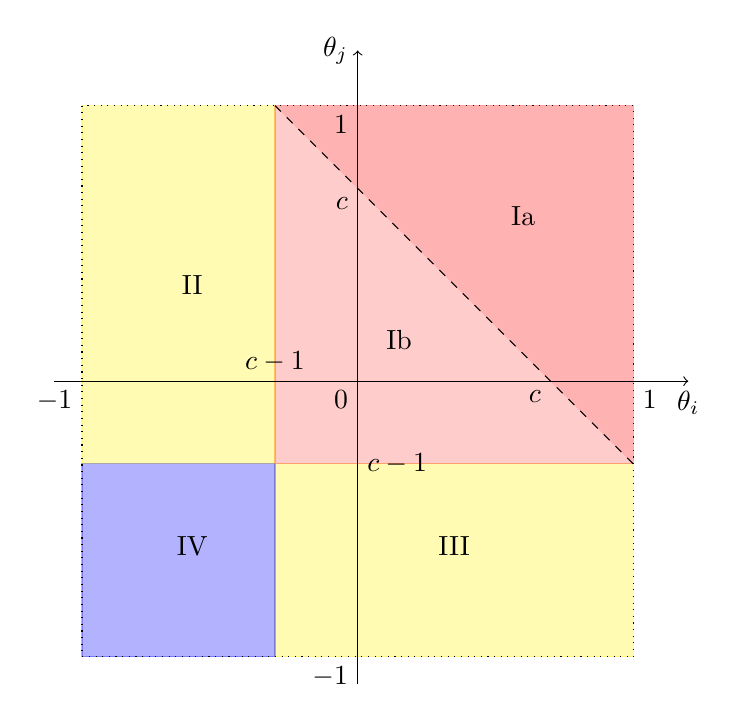
\begin{tikzpicture}[scale=3.5]
			%regions
			\filldraw[yellow, opacity=0.3] (-0.3,-0.3) -| (-1,1) -| (-0.3,-0.3);
			\filldraw[yellow, opacity=0.3] (-0.3,-0.3) -| (1,-1) -| (-0.3,-0.3);
			\filldraw[red, opacity=0.3] (-0.3,1) -| (1,1) -| (1,-0.3);
			\filldraw[red, opacity=0.2] (-0.3,1) -| (-0.3,-0.3) -| (1,-0.3);
			\filldraw[blue, opacity=0.3] (-0.3,-0.3) -| (-1,-1) -| (-0.3,-0.3);
			\draw (0.6,0.6) node{Ia};
			\draw (0.15,0.15) node{Ib};
			\draw (-0.6,0.35) node{II};
			\draw (0.35,-0.6) node{III};
			\draw (-0.6,-0.6) node{IV};
			
			% axes 
			\draw[->] (-1.1,0) -- (1.2,0) node[below]{$\theta_i$};
			\draw[->] (0,-1.1) -- (0,1.2) node[left]{$\theta_j$};
			\draw (0,0) node[below left]{$0$};
			\draw (0,1) node[below left]{$1$};
			\draw (0,-1) node[below left]{$-1$};
			\draw (1,0) node[below right]{$1$};
			\draw (-1,0) node[below left]{$-1$};
			
			\draw (-0.3,0) node[above ]{$c-1$};
			\draw (0,-0.3) node[right ]{$c-1$};
			\draw (0.7,0) node[below left]{$c$};
			\draw (0,0.7) node[below left]{$c$};
			
			% bounding box
			\draw[dotted] (1,-1) |- (-1,1) |- (1,-1);
			
			% lines
			\draw[dashed] (-0.3,1) -- (1,-0.3);
		\end{tikzpicture}
		\caption{regions for AGV transfers}
		\label{fig:AGV}
	\end{center}
\end{figure}

The regions are plotted in Figure \ref{fig:AGV}. Note that the public project is implemented only in region Ia, but the two agents' transfers sum up to zero there, same as in all other regions. Therefore, the AGV mechanism does not cover the project cost.
At this point you might think that this is because you need to compute $\tilde{t}_0$ and somehow include it in the players' payments. However, regardless of how you split this $\tilde{t}_0$ across agents, payments in regions Ia and Ib will always be continuous at the border (since $\tilde{t}]_0$ would just add some constant to agents' payments), whereas to cover the cost of the project exactly, the sum of payments must be larger by $c$ in Ia than in Ib.
%\begin{align*}
%\tilde{t}_0 &= \mathbb{E}_{\theta_1,\theta_2} \left[ (\theta_1+\theta_2) \mathbb{I} \{ \theta_1+\theta_2 \geq c \} \right]
%\\
%&= \int_{c-1}^1 \left[ \int_{c-\theta_i}^1 (\theta_1+\theta_2) d\theta_2 \right] d\theta_1 
%\\
%&= \frac{4+c^3}{3}.
%\end{align*}



%%-----------------------------------------------------------------------------------------------------

\end{document}
